\documentclass[11pt]{article}

% Anonymous review version; change to "final" for the camera-ready version.
\usepackage[review]{acl}

\usepackage{times}
\usepackage{latexsym}
\usepackage[T1]{fontenc}
\usepackage[utf8]{inputenc}
\usepackage{microtype}
\usepackage{inconsolata}
\usepackage{graphicx}
\usepackage{booktabs}
\usepackage{amsmath}

\title{What Do Linguistic Feature Groups Contribute to Early Depression Detection?\\
A Repeated Cross-Validation and Error Analysis on Reddit Users}

\author{Anonymous ACL submission}

\begin{document}
\maketitle

\begin{abstract}
Early depression detection systems are usually compared on a single split with few positive users, so it remains unclear what individual linguistic features contribute, how early they help, and which users they fail on.
We analyse feature groups (PHQ-9 item similarity, LIWC categories, language style matching, parent-text similarity, posting behaviour) with a shared causal Transformer, using 5$\times$3 repeated cross-validation over 891 Reddit users (102 labelled depressed), alarm rules chosen only on training users, and family-wise corrected paired tests.
PHQ-9 similarity is the strongest single group (ROC-AUC 0.952, PR-AUC 0.742) and is significantly better than both style-matching variants; its advantage over LIWC is smaller and less robust across tests, and groups added to it give no significant gain.
A control that knows only post position and volume already reaches ROC-AUC 0.662.
Text-based groups rank users after one post, whereas style matching needs several.
An adapter-tuned MentalRoBERTa has the best scores (ROC-AUC 0.963) and is better than TF-IDF and, more narrowly, frozen embeddings, but its advantage over a 74-feature combination is not significant after correction.
Users missed by the stronger groups have little mental-health vocabulary in their histories, a pattern we describe without a causal claim.
Because labels come from self-reported diagnoses, ``early'' means after fewer posts, not before disclosure or onset.
\end{abstract}

\section{Introduction}

Early risk detection asks a system to read a user's writings in order and to raise an alarm as soon as there is enough evidence of a condition.
The eRisk lab has run such tasks on Reddit users since 2017 \citep{losada2017erisk,losada2018overview}, and its 2025 edition introduced a contextualised early depression detection task \citep{parapar2025overview}.
Systems range from classifiers over hand-crafted linguistic features \citep{trotzek2020utilizing} to fine-tuned Transformers, but they are typically compared on one train/test split that contains a few dozen positive users.
On such splits, differences of a few points in F1 cannot be resolved, and it is rarely clear which linguistic signals a system actually relies on.

Three properties of the data make the question harder.
First, positives are rare: the collection we use has 102 depressed users among 891.
Second, depressed users write much more: the median depressed user has 525 posts, the median control user 216.
Position and volume of posts are therefore informative on their own, and any claim about a linguistic feature needs a control that knows nothing but position and volume.
Third, labels come from self-reported diagnoses, so errors are not necessarily model errors, and the kinds of users that features miss or wrongly flag are informative about what the features measure.
Throughout, \emph{depressed} and \emph{control} denote these collection labels, not independently established clinical states \citep{chancellor2020methods}, and the disclosure statements remain in the histories: \emph{early} means after fewer observed posts, not before disease onset or before a user's first disclosure.

We separate three kinds of evidence that can lead to different conclusions: \emph{standalone} signal (does a group beat the control for position and volume?), \emph{incremental} signal (does it add to a stronger group?) and \emph{early} signal (is it available after few posts?).
We therefore ask four questions.
\textbf{RQ1:} which feature groups carry signal beyond post position and volume?
\textbf{RQ2:} how early does each group detect?
\textbf{RQ3:} do features beyond PHQ-9 similarity, or a fine-tuned encoder, add anything?
\textbf{RQ4:} which users does each group get wrong, and why?
To answer them, we make three contributions:
\begin{itemize}\itemsep0pt
\item an evaluation protocol that is free of leakage across folds, uses repeated cross-validation over all labelled users, selects the alarm rule only on out-of-fold predictions of the training users, and tests differences in pre-specified families with Holm correction;
\item a comparison of single feature groups and their combinations with a position-and-volume control, in terms of ranking quality, earliness (AUC after $n$ posts, alarm delay) and decision quality, with frozen and adapter-tuned MentalRoBERTa and a TF-IDF classifier as references;
\item an error analysis by feature group: which depressed users are missed and which control users are flagged, by which groups, and how this depends on the history length and on explicit self-reports.
\end{itemize}

\section{Related Work}

\paragraph{Early detection in eRisk.}
The eRisk collection pairs Reddit users with labels derived from explicit mentions of a diagnosis and introduced the ERDE measure of early-detection performance \citep{losada2016test}; the lab has since repeated depression tasks and added others \citep{losada2017erisk,losada2018overview,parapar2022overview,parapar2025overview}.
\citet{sadeque2018measuring} proposed a latency-weighted F1, which we use.
Early detection systems include the text classification framework of \citet{burdisso2019text} and neural networks with linguistic metadata \citep{trotzek2020utilizing}; we use a causal Transformer over per-post features so that the alarm rule can be applied to a probability after every post.

\paragraph{Linguistic and psychometric signals.}
\citet{decho2013predicting} predicted depression from social media with behavioural and linguistic features, and \citet{coppersmith-etal-2014-quantifying} and \citet{yates-etal-2017-depression} built corpora around self-reported diagnoses.
We use signals with a psychological motivation: similarity to the items of the PHQ-9 questionnaire \citep{kroenke2001phq}, scored with the embedding-similarity item scoring of \citet{lahnala2025unifying}; category rates from LIWC \citep{pennebaker2015liwc}; and language style matching between a comment and the text it replies to \citep{ireland2010language}.
Mental-health encoders such as MentalRoBERTa \citep{ji-etal-2022-mentalbert} and parameter-efficient adapters \citep{houlsby2019parameter,pfeiffer-etal-2020-adapterhub,poth-etal-2023-adapters} serve as references.

\paragraph{Validity of evaluation.}
Proxy labels have limited external validity \citep{ernala2019methodological,harrigian-etal-2020-models}, available datasets differ in quality \citep{harrigian-etal-2021-state}, and studies rarely validate their methodology \citep{chancellor2020methods}.
On the statistical side, small samples give large error bars \citep{varoquaux2018cross}, paired tests need care when training sets overlap \citep{dietterich1998approximate,nadeau2003inference,demsar2006statistical}, and selecting a configuration on the data used for evaluation biases the estimate \citep{cawley2010overfitting}.
We follow these recommendations with repeated cross-validation, a selection of the alarm rule that never uses held-out users, and paired tests with multiplicity correction.

\section{Data and Task}

\paragraph{Data.}
We use the labelled collection released for eRisk 2025 Task~2: Reddit users with the submissions and comments they wrote, the text they replied to, and a label stating whether the user explicitly mentioned a depression diagnosis \citep{parapar2025overview}.
The release has 909 users; we drop empty and posts whose text was removed or deleted, after which 18 control users have no post left, giving 891 users (102 depressed) and 343{,}153 posts, without truncation or down-sampling.
Table~\ref{tab:data} summarises the data.
Depressed users write more posts, longer posts, over longer periods, and more of their posts are comments with a known parent text.

\begin{table}[t]
\centering\footnotesize
\resizebox{\columnwidth}{!}{%
\begin{tabular}{lrr}
\toprule
 & Depressed & Control \\
\midrule
Users & 102 & 789 \\
Posts & 66{,}679 & 276{,}474 \\
Posts per user, median [IQR] & 525 [131, 1005] & 216 [50, 705] \\
Words per post, median & 22 & 13 \\
Comments among posts & 93.4\% & 89.6\% \\
Posts with parent text & 64.0\% & 59.3\% \\
Time span (days), median & 1181 & 388 \\
Users with a self-report phrase & 83 (81\%) & 27 (3.4\%) \\
\bottomrule
\end{tabular}}
\caption{Data. ``Self-report phrase'': at least one post matching a first-person pattern such as ``I was diagnosed with depression'' (Appendix~\ref{app:sr}).}
\label{tab:data}
\end{table}

\paragraph{Task and alarm rule.}
After each post $t$ the system outputs a probability $p_t$ that the user is depressed.
An alarm is raised at the first post $d$ such that $p_{d-k+1},\dots,p_d\ge\theta$, and $d$ is the delay; users without an alarm are predicted negative.
The pair $(\theta,k)$ is chosen with $\theta\in\{0.05,\dots,0.95\}$ and $k\in\{1,3,5,10\}$ to maximise the latency-weighted F1,
\begin{equation*}
F_{\mathrm{lat}} = F_1\cdot\bigl(1-\operatorname{median}_{\text{TP}}\,(-1+\tfrac{2}{1+e^{-\rho (d-1)}})\bigr),
\end{equation*}
with $\rho=0.0078$ as in eRisk \citep{sadeque2018measuring}, where the median is over detected depressed users.
We also report ROC-AUC and PR-AUC of the maximum probability of a user, AUC after $n$ posts (the probability after $n$ posts, or after the last post for users with fewer), the share of users flagged within $n$ posts, precision, recall, F1 and the median delay.

\section{Features and Models}

\paragraph{Per-post feature groups.}
Every group is described by features of the current post plus history features (running maximum and minimum, their difference, change from the previous post, rolling standard deviation over 5 posts, running mean), standardised with training statistics and clipped to $\pm10$.
\textbf{PHQ} (28 features including context): cosine similarity between a post and nine first-person archetype sentences, one per PHQ-9 item (Appendix~\ref{app:phq}), computed with mxbai-embed-large-v1 \citep{lee2024mxbai,li2023angle} following \citet{lahnala2025unifying}, their mean, and running maxima per item.
These are similarities inspired by symptoms, not observed PHQ responses or validated estimates of severity.
\textbf{LIWC} (33): rates of 15 categories in the post's own text (e.g.\ sadness, anxiety, health, negative emotion, first-person singular) from LIWC2015 \citep{pennebaker2015liwc}.
\textbf{LSM} (73): language style matching \citep{ireland2010language} between a comment and its parent on ten LIWC-based scores, $1-|a-b|/(a+b+\epsilon)$ per category, computed on word counts, as in our initial pipeline, which mixes in text length.
\textbf{LSM alignment} (43): the same score on word rates, plus the signed difference of the group rates between comment and parent.
\textbf{Cosine similarity} (10): similarity of sentence embeddings (all-MiniLM-L6-v2; \citealp{reimers-gurevych-2019-sentence}) between a comment and its parent.
\textbf{Behaviour} (9): log word count, posting between 00:00 and 05:59 UTC, log time since the previous post.
LSM, alignment and cosine similarity exist only for comments whose parent text is known (about 60\% of the rows).
In every single-group run we add three \textbf{context} features: log post index, comment indicator and parent-known indicator.
\textbf{Context only} uses just these three and is our control for position and volume.

\paragraph{Style matching.}
For a comment and its parent, count LSM scores each LIWC category $c$ with word counts $a_c,b_c$ as $1-|a_c-b_c|/(a_c+b_c+\epsilon)$ and averages the categories into ten groups $G$ (function words, social, positive, negative, four person and pronoun groups, cognitive, perceptual).
The alignment variant uses category rates $r_c$ (comment) and $q_c$ (parent):
\begin{align*}
m_G &= \tfrac{1}{|G|}\textstyle\sum_{c\in G}\bigl(1-\tfrac{|r_c-q_c|}{r_c+q_c+10^{-6}}\bigr),\\
\delta_G &= \tfrac{1}{|G|}\textstyle\sum_{c\in G}(r_c-q_c).
\end{align*}
Two zero rates give a score of one, which can make sparse texts look aligned, and normalisation does not remove topical or interaction-selection effects.
Counts mix in text length; we keep this variant as an empirical comparator, not as canonical LSM.

\paragraph{Sequence model.}
A linear projection feeds a 3-layer Transformer encoder (hidden size 256, 4 heads, dropout 0.3, 4.0M parameters) with a causal mask, so the output after post $t$ depends only on posts $1..t$ \citep{vaswani2017attention}.
It is trained with a per-post binary cross-entropy against the user label, each user weighted equally, a class weight equal to the ratio of negative to positive users, AdamW \citep{loshchilov2017decoupled} (learning rate $3\cdot10^{-5}$) and early stopping on 12\% of the training users.

\paragraph{Reference systems.}
\textbf{Frozen MentalRoBERTa}: mean-pooled last-layer embeddings (768 dimensions) of each post, used in place of the hand-crafted features.
\textbf{Adapter-tuned MentalRoBERTa}: a bottleneck adapter and classification head on the same encoder, trained on posts with the user label (3 epochs, at most 200 posts per user and epoch); its logit is the only input apart from the context features.
\textbf{TF-IDF}: word 1--2-gram TF-IDF with logistic regression on posts; the user score after $n$ posts is the running mean of the post logits.
\textbf{Self-report rule}: no learning; an alarm at the first post that matches the self-report pattern.
It is not a model of depression but shows what the labelling alone yields.

\section{Evaluation Protocol}

We pool the 891 users and run stratified 5-fold cross-validation three times (15 outer folds).
In each outer fold the sequence model is trained exactly as above on the outer training users with an inner 5-fold cross-validation; the pooled inner out-of-fold probabilities of the training users select $(\theta,k)$, and the five inner models are averaged on the held-out users.
Every user is therefore predicted once per repeat by models that never saw it, and the rule is never tuned on held-out users \citep{cawley2010overfitting}.
Components fitted with labels are refitted inside every outer fold: the adapter is retrained on the outer training users (three inner models) and the TF-IDF classifier is refitted.
A relative-entropy feature from language models fitted on depressed and control posts would need the same nested refitting and is not used.
All configurations share splits and seeds.

Metrics are means over the three repeats, with 95\% intervals from a stratified bootstrap over users (2000 draws, identical for all configurations, repeats averaged inside each draw).
Differences are tested in three pre-specified families (9 comparisons among references; 4 against the TF-IDF baseline; 9 among feature groups and against the control) with two-sided bootstrap $p$-values of the mean difference and Holm adjustment inside each family.
Nadeau--Bengio corrected resampled $t$-tests, DeLong tests and McNemar tests are in Appendix~\ref{app:pairs}.
Error analysis uses the decisions of the three repeats: a user is an error of a configuration if it is misclassified in at least two of them.

\section{Results}

\subsection{Which feature groups carry signal (RQ1)}

\begin{table*}[t]
\centering\small
\begin{tabular}{lrccccc}
\toprule
Configuration & \#feat. & ROC-AUC & PR-AUC & AUC@10 & F1 & F$_{\mathrm{lat}}$ \\
\midrule
\multicolumn{7}{l}{\textit{Single feature groups (plus three context features)}} \\
PHQ & 28 & .952 [.935, .968] & .742 [.677, .815] & .875 & .718 & .681 \\
LIWC (15 categories) & 33 & .926 [.901, .949] & .660 [.586, .745] & .847 & .653 & .620 \\
LSM (counts) & 73 & .874 [.837, .909] & .556 [.476, .641] & .764 & .564 & .479 \\
LSM alignment & 43 & .851 [.811, .886] & .478 [.403, .568] & .745 & .507 & .464 \\
Behaviour & 9 & .808 [.763, .849] & .375 [.314, .458] & .745 & .438 & .416 \\
Cosine similarity & 10 & .727 [.676, .778] & .303 [.244, .381] & .621 & .272 & .255 \\
Context only (control) & 3 & .662 [.607, .718] & .333 [.259, .419] & .620 & .236 & .225 \\
\midrule
\multicolumn{7}{l}{\textit{Combinations and reference systems}} \\
PHQ + 3 LIWC categories & 34 & .952 [.934, .968] & .749 [.679, .820] & .891 & .732 & .706 \\
PHQ + 3 LIWC + 4 LSM scores & 42 & .958 [.942, .974] & .777 [.710, .846] & .892 & .751 & .713 \\
PHQ + 3 LIWC + LSM alignment & 74 & .953 [.934, .970] & .753 [.689, .822] & .883 & .723 & .680 \\
MentalRoBERTa, frozen & 771 & .938 [.914, .960] & .726 [.659, .798] & .889 & .729 & .708 \\
MentalRoBERTa, adapter-tuned & 4 & .963 [.947, .977] & .792 [.732, .852] & .878 & .788 & .762 \\
TF-IDF + logistic regression & -- & .914 [.884, .940] & .680 [.601, .759] & .902 & .715 & .702 \\
First self-report phrase (no learning) & -- & .897 & .754 & .578 & .783 & .621 \\
\bottomrule
\end{tabular}

\caption{5$\times$3 cross-validation over 891 users (102 depressed): mean over repeats with 95\% bootstrap intervals for ROC-AUC and PR-AUC (prevalence 0.114); AUC@10 intervals are about $\pm$0.04. \#feat.\ includes three context features. F$_{\mathrm{lat}}$ is the latency-weighted F1. The last row is not a cross-validated model.}
\label{tab:results}
\end{table*}

Table~\ref{tab:results} ranks the groups: PHQ (ROC-AUC .952, PR-AUC .742) $>$ LIWC (.926, .660) $>$ LSM counts (.874, .556) $>$ LSM alignment (.851, .478) $>$ behaviour (.808, .375) $>$ cosine similarity (.727, .303).
PHQ is better than LIWC (ROC $+.027$, PR $+.082$; Holm $p=.004$ and $.024$), than LSM counts and than LSM alignment (PR $+.186$ and $+.264$; $p=.004$).
Every group exceeds the context-only control in ROC-AUC (Holm $p\le.018$), but in PR-AUC only PHQ, LIWC and the two LSM variants do ($p\le.042$); behaviour and cosine similarity do not ($p=.686$).
The control matters: position and volume alone reach ROC-AUC .662 and PR-AUC .333, and its decision rule flags 583 of the 789 control users (precision .137).
The differences in ROC-AUC between PHQ and the other groups, and between each group and the control, also hold under the Nadeau--Bengio test; the PR-AUC and F1 differences between PHQ and LIWC are significant only under the bootstrap test, so we regard them as suggestive (Appendix~\ref{app:pairs}).

\subsection{How early each group detects (RQ2)}

\begin{figure*}[t]
\centering
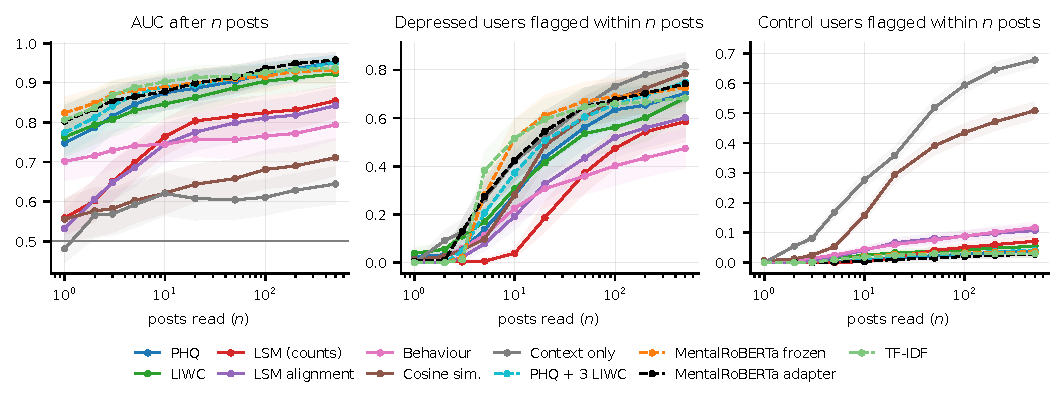
\includegraphics[width=\textwidth]{fig_curves.pdf}
\caption{Left: AUC after $n$ posts. Middle and right: share of depressed and of control users flagged within $n$ posts under the rule chosen in each outer fold. Solid: single feature groups; dashed: references. Bands: 95\% bootstrap intervals.}
\label{fig:curves}
\end{figure*}

\begin{table*}[t]
\centering\small
\resizebox{0.85\textwidth}{!}{\begin{tabular}{lccccc}
\toprule
Configuration & AUC@1 & AUC@10 & Flagged $\leq$10 & Precision & Median delay [Q1--Q3] \\
\midrule
PHQ & .748 & .875 & .281 & .699 & 14.0 [10--46] \\
LIWC & .763 & .847 & .307 & .613 & 14.0 [6--45] \\
LSM (counts) & .559 & .764 & .039 & .517 & 40.0 [17--96] \\
LSM alignment & .532 & .745 & .193 & .421 & 22.8 [8--74] \\
Behaviour & .702 & .745 & .226 & .365 & 14.2 [6--120] \\
Cosine sim. & .556 & .621 & .281 & .163 & 17.0 [9--54] \\
Context only & .481 & .620 & .422 & .137 & 12.5 [4--52] \\
PHQ + 3 LIWC & .774 & .891 & .372 & .700 & 10.3 [5--35] \\
MentalRoBERTa frozen & .824 & .889 & .516 & .722 & 8.3 [5--12] \\
MentalRoBERTa adapter & .803 & .878 & .425 & .783 & 9.5 [5--32] \\
TF-IDF & .806 & .902 & .516 & .749 & 5.7 [5--10] \\
First self-report phrase & -- & .578 & -- & .754 & 55 [--] \\
\bottomrule
\end{tabular}
}
\caption{Earliness. Flagged $\leq$10: share of all depressed users flagged within 10 posts. Precision and delay are over the decisions of the chosen rule; delay is over detected depressed users.}
\label{tab:early}
\end{table*}

After a single post (Figure~\ref{fig:curves}, left; Table~\ref{tab:early}), LIWC (AUC .763) and PHQ (.748) already rank users, as do behaviour (.702) and the two references that read the post text (.80--.82), whereas LSM, LSM alignment and cosine similarity are at .53--.56: they exist only for comments with a known parent and need several posts to accumulate.
At 10 posts PHQ reaches .875 and LIWC .847; at 100 posts PHQ (.922) is close to the adapter-tuned encoder (.936).
Among the informative groups, LIWC alarms earliest (median delay 14 posts, 44\% of its detected users within 10 posts) but is less precise than PHQ (.613 against .699); LSM counts is slowest (median 40 posts).
The combination of PHQ and three LIWC categories alarms earlier than either (median 10.3 posts) at PHQ's precision, but this is descriptive: we do not test delay differences.
TF-IDF and the encoders alarm earliest (median 5.7 to 9.5 posts).
After 500 posts the false-alarm rate on control users is under 6\% for PHQ and LIWC, about 11\% for behaviour and LSM alignment, and 68\% for the context-only rule (Figure~\ref{fig:curves}, right).

\subsection{Beyond PHQ, and encoders (RQ3)}

\begin{table}[t]
\centering\footnotesize
\resizebox{\columnwidth}{!}{\begin{tabular}{lccc}
\toprule
Comparison (A $-$ B) & $\Delta$ROC & $\Delta$PR & $\Delta$F1 \\
\midrule
PHQ $-$ LIWC & +.027 (.004) & +.082 (.024) & +.064 (.017) \\
PHQ $-$ LSM (counts) & +.078 (.004) & +.186 (.004) & +.154 (.004) \\
PHQ $-$ LSM alignment & +.102 (.004) & +.264 (.004) & +.211 (.004) \\
74 feat. $-$ PHQ & +.001 (1) & +.010 (1) & +.005 (1) \\
74 feat. $-$ PHQ+3 LIWC+4 LSM & $-$.005 (.042) & $-$.025 (.322) & $-$.028 (.182) \\
Adapter $-$ frozen & +.024 (.004) & +.065 (.045) & +.059 (.018) \\
Adapter $-$ TF-IDF & +.049 (.002) & +.111 (.002) & +.073 (.004) \\
Adapter $-$ 74 feat. & +.010 (.192) & +.039 (.810) & +.065 (.088) \\
\bottomrule
\end{tabular}
}
\caption{Key paired differences (mean over repeats; Holm-adjusted $p$ in parentheses). All 22 comparisons are in Appendix~\ref{app:pairs}.}
\label{tab:key}
\end{table}

Adding three LIWC categories to PHQ, additionally four LSM scores, or the LSM alignment features (74 features in total) does not change ROC-AUC or PR-AUC significantly relative to PHQ alone (74 features against PHQ: $\Delta$ROC $+.001$, $\Delta$PR $+.010$, Holm $p=1$; Tables~\ref{tab:results} and~\ref{tab:key}).
The four-score variant is slightly better than the alignment variant in ROC-AUC (Holm $p=.042$, not significant under Nadeau--Bengio).
The adapter-tuned MentalRoBERTa is best overall (ROC-AUC .963, PR-AUC .792, F1 .788).
It is better than TF-IDF ($\Delta$ROC $+.049$, $\Delta$PR $+.111$, $\Delta$F1 $+.073$; Holm $p\le.004$) and, more narrowly, than frozen embeddings ($+.024$, $+.065$, $+.059$; $p=.004$, $.045$, $.018$; the PR-AUC difference has Nadeau--Bengio $p=.057$).
Against the 74-feature hand-crafted set the difference is borderline: $\Delta$ROC $+.010$, $\Delta$PR $+.039$, $\Delta$F1 $+.065$, with unadjusted bootstrap $p=.032$, $.135$, $.011$ and Holm $p=.19$, $.81$, $.088$.
This does not establish equivalence: an F1 gap of .065 may matter in practice.
TF-IDF ranks users worse (ROC-AUC .914) but has the highest AUC@10 (.902) and the shortest delay.
The self-report rule reaches F1 .783, close to the adapter-tuned model (.788), but alarms much later (median 55 posts against 9.5): the learned models mainly gain earliness.

\subsection{Errors by feature group (RQ4)}

\begin{figure*}[t]
\centering
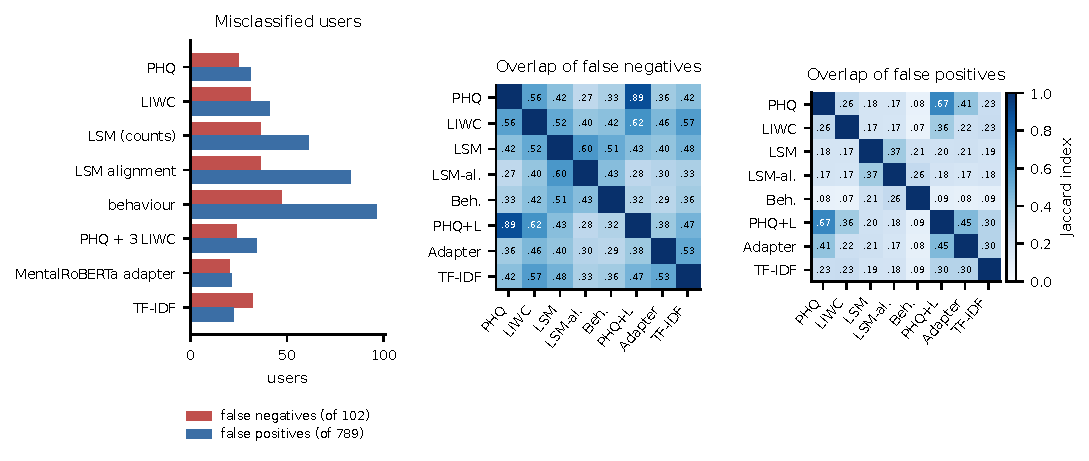
\includegraphics[width=\textwidth]{fig_errors.pdf}
\caption{Left: misclassified users per configuration. Middle and right: overlap (Jaccard index) of the sets of false negatives and of false positives.}
\label{fig:errors}
\end{figure*}

\begin{table*}[t]
\centering\small
\resizebox{0.85\textwidth}{!}{\begin{tabular}{lccccccccc}
\toprule
& & & \multicolumn{3}{c}{False negatives} & \multicolumn{2}{c}{False positives} & \multicolumn{2}{c}{Recall by self-report} \\
\cmidrule(lr){4-6}\cmidrule(lr){7-8}\cmidrule(lr){9-10}
Configuration & FN & FP & Posts & MH & SR & Posts & SR & with & without \\
\midrule
PHQ & 25 & 31 & 622 & 5.1\% & 64\% & 412 & 23\% & 0.81 & 0.53 \\
LIWC & 31 & 41 & 622 & 5.3\% & 58\% & 231 & 20\% & 0.78 & 0.32 \\
LSM (counts) & 36 & 61 & 546 & 9.5\% & 67\% & 483 & 18\% & 0.71 & 0.37 \\
LSM alignment & 36 & 83 & 304 & 11.5\% & 67\% & 368 & 13\% & 0.71 & 0.37 \\
Behaviour & 47 & 96 & 336 & 12.6\% & 72\% & 660 & 7\% & 0.59 & 0.32 \\
PHQ + 3 LIWC & 24 & 34 & 746 & 3.1\% & 62\% & 416 & 21\% & 0.82 & 0.53 \\
MentalRoBERTa adapter & 20 & 21 & 854 & 2.8\% & 60\% & 241 & 38\% & 0.86 & 0.58 \\
TF-IDF & 32 & 22 & 954 & 3.2\% & 69\% & 172 & 27\% & 0.73 & 0.47 \\
\bottomrule
\end{tabular}
}
\caption{Misclassified users (wrong in $\ge2$ of 3 repeats). Posts: median posts per user; SR: share with a self-report phrase. Recall is split by whether a depressed user has a self-report phrase (83 users) or not (19 users).}
\label{tab:errors}
\end{table*}

The groups err on different users (Figure~\ref{fig:errors}).
The false-negative sets overlap strongly between PHQ and PHQ with LIWC (Jaccard .89, the combination mostly inherits PHQ's misses), moderately between PHQ and LIWC (.56), and little between PHQ and LSM alignment (.27) or the adapter-tuned model (.36); false-positive sets overlap much less (.07 to .26 between groups).

\paragraph{False negatives.}
Users missed by the stronger groups have long histories with sparse evidence: the median is 622 posts for PHQ and LIWC (854 for the adapter), and only 5\% of their posts contain mental-health terms (adapter: 2.8\% against 15.5\% for its true positives, unadjusted $p<.001$).
The history length itself does not differ significantly between the adapter's false negatives and true positives (854 against 464 posts, $p=.236$), so this is an evidence-density pattern, not a demonstrated effect of length.
Reading the highest-scoring posts of the 20 users missed by the adapter-tuned model, 17 contain a first-person statement of a diagnosis or of ongoing depression, which the post-level model scores highly; the sequence model does not keep such isolated evidence, and 15 of the 20 never reach the threshold.
Weaker groups also miss users with shorter histories (304 posts for LSM alignment, 336 for behaviour).

\paragraph{False positives.}
Semantic groups flag control users who write about depression: 23\%, 20\% and 18\% of the false positives of PHQ, LIWC and LSM match the self-report pattern, against 3.4\% of all control users (adapter: 38\%).
In a reading of the false positives of the adapter-tuned model and of the 74-feature set, most flagged users describe their own depression, another condition, a chronic illness, everyday distress, or support others in mental-health communities (Appendix~\ref{app:errors}).
Behaviour flags heavy posters (median 660 posts against 207 for true negatives; 7\% self-reports).
The alarm is usually raised on an unremarkable post and reflects the accumulated history.

\paragraph{History length.}
Table~\ref{tab:length} splits the users by the number of posts.
The recall of the systems that score post text falls as histories grow (TF-IDF .87, .76, .57; frozen encoder .91, .80, .67; adapter .87, .84, .76), which is consistent with evidence dilution, whereas PHQ and LIWC are weak on short histories (.61 below 100 posts, against .87 to .91 for the text systems) and best at 100--499 posts (.88 and .76).
Features that accumulate over the history thus need a minimum of posts, and text systems lose evidence in long ones.
With 23, 25 and 54 depressed users per bin these values are indicative.

\begin{table}[t]
\centering\footnotesize
\resizebox{\columnwidth}{!}{\begin{tabular}{lccc}
\toprule
Posts per user & <100 (23/280) & 100--499 (25/243) & $\geq$500 (54/266) \\
\midrule
PHQ & .609 (.021) & .880 (.053) & .759 (.045) \\
LIWC & .609 (.050) & .760 (.062) & .704 (.045) \\
LSM (counts) & .391 (.029) & .840 (.099) & .667 (.109) \\
LSM alignment & .435 (.071) & .760 (.132) & .685 (.117) \\
Behaviour & .391 (.050) & .480 (.128) & .630 (.192) \\
PHQ + 3 LIWC & .696 (.021) & .880 (.058) & .741 (.053) \\
MentalRoBERTa frozen & .913 (.032) & .800 (.058) & .667 (.026) \\
MentalRoBERTa adapter & .870 (.014) & .840 (.041) & .759 (.026) \\
TF-IDF & .870 (.025) & .760 (.049) & .574 (.011) \\
\bottomrule
\end{tabular}
}
\caption{Recall of depressed users (false-alarm rate of control users) by number of posts per user (depressed/control users in parentheses); decisions as in Table~\ref{tab:errors}.}
\label{tab:length}
\end{table}

\paragraph{Self-reports.}
Depressed users without a self-report phrase are harder for every configuration (19 users, so values are indicative): recall falls from .81 to .53 for PHQ, from .86 to .58 for the adapter-tuned model, and more for LIWC (.78 to .32) and behaviour (.59 to .32).

\section{Discussion}

Standalone, incremental and early signal lead to different conclusions.
Style matching improves over the control but not demonstrably over PHQ with LIWC; PHQ leads the single groups in full-history ranking, whereas TF-IDF has the highest AUC@10 among the references; a ranking winner need not be an early-alarm winner.
PHQ similarity is the strongest and among the earliest signals, and it gains nothing from the other groups we tested.
This is consistent with its construction: it scores each post against symptom statements and therefore responds to symptom-like content from the first post on.
LIWC categories give a coarser lexical version of this signal.
Style matching and parent similarity are properties of an exchange, are undefined for submissions and for comments without a parent, and need several posts; they also add little to PHQ.
Behaviour and context mostly reflect how much a user writes; a control for this is necessary, since position and volume alone give ROC-AUC .662.

That a control for position and volume is needed echoes the concern that confounding factors can lead to an overestimate of performance on social-media mental-health data \citep{harrigian-etal-2020-models}; here the control is cheap, since the three context features are available in every setting.
The two families depend differently on the history length (Table~\ref{tab:length}), but a simple concatenation of the adapter logit and the 74 hand-crafted features did not improve on the adapter alone ($\Delta$PR $-.020$, Holm $p=1$; Appendix~\ref{app:pairs}).
For early detection systems, the error analysis suggests two directions that we did not test: aggregation that keeps the strongest evidence instead of an average-like summary (misses are users with a few strong posts in long histories), and a distinction between writing about depression and having it (many false positives come from mental-health communities).
Because labels are derived from self-reported diagnoses, the results describe the detection of users who have disclosed a diagnosis; a rule that only looks for the disclosure reaches an F1 close to the best model and differs mainly in delay, so absolute F1 values should be read with the labelling in mind.

\section{Conclusion}

In a repeated cross-validation over 891 Reddit users, PHQ-9 item similarity is the strongest single feature group, features beyond it add no significant gain, post position and volume are a necessary control, text-based groups detect from the first post whereas style matching needs several, and an adapter-tuned encoder is best but not significantly better than hand-crafted features after correction.
Groups fail on different users, but distinct errors do not guarantee useful fusion: adding the hand-crafted features does not improve the adapter.
Misses are associated with sparse mental-health evidence in long histories (recall of the text systems falls as histories grow), and false alarms with topic; both are descriptive.
The results support feature analysis, not a claim of state-of-the-art detection, and they concern users who disclosed a diagnosis.

\section*{Limitations}

The collection has 102 depressed users from one platform, so intervals are wide (about $\pm0.07$ in PR-AUC), non-significant differences are not evidence of equality, and the findings may not transfer to other data.
Labels come from self-reported diagnoses; control users are not verified as non-depressed, and some describe their own depression.
We use one sequence-model seed and one adapter run per outer fold; hyper-parameters and the feature groups were chosen earlier on users who are part of the cross-validation, which favours those choices.
The alarm rule is chosen on single-model out-of-fold probabilities but applied to averaged models, which may shift threshold-based metrics slightly.
A relative-entropy feature is not evaluated because it needs nested refitting.
The categories of errors come from one reader who read the highest-scoring posts of each user, and the keyword patterns are not validated.
Delay differences are descriptive and involve different sets of detected users.
Peak ranking rewards observation opportunity, and fixed-prefix AUC keeps the final score of shorter histories instead of using a common-length cohort.
Adapter logits are cross-fitted inside each outer training set and reused across the classifier's inner folds, so the inner procedure is not a fully nested end-to-end selection.
PHQ extraction uses a 335M-parameter encoder, so a compact feature vector does not mean lower inference cost than MentalRoBERTa.
We do not evaluate on the official eRisk test servers, which provide full conversational context.

\section*{Ethical Considerations}

The data were obtained under the eRisk 2025 user agreement; we quote no posts and report only aggregate statistics.
Depression detection can harm users through false accusations, exposure and misuse for profiling.
Our results are for research on evaluation; the systems must not be used to screen, label or monitor people, and they do not provide a diagnosis.
Code will be released without data and without the LIWC dictionary, which is licensed separately.

\bibliography{refs}

\appendix

\section{PHQ-9 Archetype Sentences}
\label{app:phq}

We wrote one first-person sentence per PHQ-9 item; the PHQ feature of a post is the cosine similarity between the embedding of the post and the embedding of each sentence:
(1) \emph{I haven't been wanting to do anything.}
(2) \emph{I've been feeling really low lately.}
(3) \emph{I can't sleep properly---either too little or too much.}
(4) \emph{I barely have any energy to do things.}
(5) \emph{My appetite is totally messed up.}
(6) \emph{I feel like I'm not good enough.}
(7) \emph{I can't focus on anything for long.}
(8) \emph{I feel like I'm moving in slow motion.}
(9) \emph{I just feel like giving up sometimes.}

\section{Implementation Details}
\label{app:impl}

\paragraph{Sequence model and training.}
Input projection to 256 dimensions, 3 Transformer encoder layers (4 heads, feed-forward width 2048, dropout 0.3), a two-layer head (256$\rightarrow$64$\rightarrow$1) producing one logit per post, no positional encoding (order enters through the causal mask and the post-index feature), at most 30 epochs, patience 5, weight decay 0.01, gradient clipping 1.0, length-bucketed batches of at most 32 users.
Hyper-parameters (learning rate $3\cdot10^{-5}$, 256$\times$3) were chosen on a 16-configuration grid by out-of-fold PR-AUC on the 712 training users of an earlier fixed split; the spread across the grid is about 0.075 PR-AUC.
$(\theta,k)$ is selected by $F_{\mathrm{lat}}$, ties by F1, then shorter delay, then lower threshold.

\paragraph{Adapter.}
Bottleneck adapter and a two-class head on mental/mental-roberta-base (126.8M parameters, 2.13M trained), post-level training with the user label, 3 epochs, learning rate $3\cdot10^{-4}$, batch size 32, maximum length 256, at most 200 random posts per user and epoch, best epoch chosen on 10\% of the fit users.
In the cross-validation three inner models are trained per outer fold on the outer training users; training users receive the logit of the inner model that did not see them, held-out users the mean of the three.

\paragraph{TF-IDF.}
Word 1--2-grams, minimum document frequency 5, at most 200{,}000 terms, sublinear tf, vocabulary fitted on the outer training text without labels; logistic regression ($C=1$, user-weighted, class-balanced); $C$ was fixed and not tuned.

\paragraph{Single split versus cross-validation.}
On a fixed split with 21 test positives, the 74-feature set reached PR-AUC .831 on the test users, against .753 pooled over all users in the cross-validation; single-split estimates of this kind are optimistic.

\paragraph{Artifacts and licences.}
The eRisk data are used under the lab's user agreement and are not redistributed.
LIWC2015 is licensed separately and not redistributed.
mental-roberta-base is used under CC BY-NC 4.0 for non-commercial research; all-MiniLM-L6-v2 and mxbai-embed-large-v1 are Apache-2.0.
Our own code and the archetype sentences will be released with the paper.

\paragraph{Compute.}
The cross-validation (15 outer folds, 17 configurations) and the adapter runs used two 24\,GB GPUs; the sequence models train in about a minute per outer fold.

\section{Paired Tests}
\label{app:pairs}

Table~\ref{tab:pairs} gives all 22 pre-specified comparisons.
Holm: bootstrap $p$-value adjusted within the family; NB: Nadeau--Bengio corrected resampled $t$-test over the 15 folds; DeLong and McNemar: median over the three repeats.
The tests agree for the main findings (PHQ against LSM and against the control; adapter against TF-IDF).
They differ for borderline comparisons: PHQ against LIWC in PR-AUC (NB $p=.209$) and F1 (McNemar $p=.060$); the adapter against the frozen encoder in PR-AUC (NB $p=.057$); the four-score variant against the alignment variant in ROC-AUC (NB $p=.215$).
We therefore describe these as suggestive.

\begin{table*}[t]
\centering\scriptsize
\resizebox{\textwidth}{!}{\begin{tabular}{llrcccrccrcc}
\toprule
Fam. & A $-$ B & $\Delta$ROC & Holm & NB & DeLong & $\Delta$PR & Holm & NB & $\Delta$F1 & Holm & McNemar \\
\midrule
1 & 74 feat. $-$ PHQ & +0.001 & 1 & .504 & .747 & +0.010 & 1 & .715 & +0.005 & 1 & .243 \\
1 & 74 feat. $-$ PHQ + 3 LIWC & +0.001 & 1 & .825 & .574 & +0.004 & 1 & .657 & $-$0.009 & 1 & .377 \\
1 & 74 feat. $-$ PHQ + 3 LIWC + 4 LSM & $-$0.005 & .042 & .215 & .066 & $-$0.025 & .322 & .269 & $-$0.028 & .182 & .180 \\
1 & 74 feat. $-$ MentalRoBERTa frozen & +0.015 & .192 & .194 & .168 & +0.027 & 1 & .925 & $-$0.006 & 1 & .392 \\
1 & 74 feat. $-$ MentalRoBERTa adapter & $-$0.010 & .192 & .032 & .096 & $-$0.039 & .810 & .033 & $-$0.065 & .088 & .019 \\
1 & MentalRoBERTa adapter $-$ MentalRoBERTa frozen & +0.024 & .004 & .024 & .004 & +0.065 & .045 & .057 & +0.059 & .018 & .041 \\
1 & Adapter + 74 feat. $-$ MentalRoBERTa adapter & $-$0.005 & 1 & .142 & .432 & $-$0.020 & 1 & .119 & $-$0.050 & .270 & .044 \\
1 & Adapter + 74 feat. $-$ 74 feat. & +0.005 & .004 & .041 & .010 & +0.019 & .192 & .080 & +0.015 & .570 & .289 \\
1 & Frozen + 74 feat. $-$ 74 feat. & +0.004 & 1 & .222 & .580 & $-$0.011 & 1 & .158 & $-$0.004 & 1 & .362 \\
2 & MentalRoBERTa adapter $-$ TF-IDF & +0.049 & .002 & $<$.001 & $<$.001 & +0.111 & .002 & .003 & +0.073 & .004 & .073 \\
2 & MentalRoBERTa frozen $-$ TF-IDF & +0.024 & .002 & .022 & .008 & +0.046 & .204 & .007 & +0.014 & 1 & 1 \\
2 & PHQ $-$ TF-IDF & +0.038 & .002 & .012 & $<$.001 & +0.062 & .204 & .061 & +0.003 & 1 & .784 \\
2 & 74 feat. $-$ TF-IDF & +0.039 & .002 & .006 & $<$.001 & +0.072 & .138 & .031 & +0.008 & 1 & .341 \\
3 & PHQ $-$ Context only & +0.291 & .004 & $<$.001 & $<$.001 & +0.409 & .004 & $<$.001 & +0.482 & .004 & $<$.001 \\
3 & LIWC $-$ Context only & +0.264 & .004 & $<$.001 & $<$.001 & +0.326 & .004 & $<$.001 & +0.417 & .004 & $<$.001 \\
3 & LSM (counts) $-$ Context only & +0.212 & .004 & $<$.001 & $<$.001 & +0.223 & .004 & .019 & +0.328 & .004 & $<$.001 \\
3 & LSM alignment $-$ Context only & +0.189 & .004 & $<$.001 & $<$.001 & +0.144 & .042 & .035 & +0.271 & .004 & $<$.001 \\
3 & Cosine sim. $-$ Context only & +0.066 & .018 & .026 & .029 & $-$0.030 & .686 & .962 & +0.036 & .004 & $<$.001 \\
3 & Behaviour $-$ Context only & +0.146 & .004 & $<$.001 & $<$.001 & +0.042 & .686 & .241 & +0.202 & .004 & $<$.001 \\
3 & PHQ $-$ LIWC & +0.027 & .004 & .014 & .007 & +0.082 & .024 & .209 & +0.064 & .017 & .060 \\
3 & PHQ $-$ LSM alignment & +0.102 & .004 & $<$.001 & $<$.001 & +0.264 & .004 & $<$.001 & +0.211 & .004 & $<$.001 \\
3 & PHQ $-$ LSM (counts) & +0.078 & .004 & .001 & $<$.001 & +0.186 & .004 & .011 & +0.154 & .004 & .007 \\
\bottomrule
\end{tabular}
}
\caption{Pre-specified paired comparisons. Families: 1 references, 2 TF-IDF baseline, 3 feature groups and control. Differences are A $-$ B, mean over repeats.}
\label{tab:pairs}
\end{table*}

\section{Self-Report Patterns}
\label{app:sr}

The self-report pattern matches first-person statements such as ``I have/had/was diagnosed with (a few words) depression'', ``my depression'', ``I'm depressed'' and ``diagnosed with (a few words) depression'' (case-insensitive).
The mental-health vocabulary pattern covers terms such as depression, anxiety, therapy, psychiatric, antidepressant, suicide, bipolar, PTSD and self-harm.
Both were fixed before the errors were inspected and are not validated; they miss phrasings such as ``I have chronic depression''.

\section{Error Categories}
\label{app:errors}

One reader assigned each false positive of the adapter-tuned model (21 users) and of the 74-feature set (34 users) to the first matching category, from the highest-scoring posts; there was no second annotator, so counts are indicative.
\emph{Own depression described in the first person}: 8 and 6;
\emph{other mental-health condition or treatment}: 4 and 9;
\emph{chronic physical illness}: 3 and 4;
\emph{everyday distress}: 4 and 9;
\emph{supportive commenters in mental-health communities}: 2 and 5;
\emph{no clear depression-related content}: 0 and 1.
Of the 20 users missed by the adapter-tuned model, 17 contain a first-person statement of a diagnosis or ongoing depression (the keyword pattern finds 12).

\end{document}
